%% 05-tripleddd.tex — Italian Stata Conference, Milano — September 2026
%% Triple differences: a design for when parallel trends breaks down
%% Ported from Causal-Inference-2/Slides/Tex/02-Codechella-Violations.tex (Triple Differences section)
%% Scott Cunningham, Baylor University
%%
%% Compile: pdflatex 05-tripleddd.tex

\documentclass[aspectratio=169,11pt]{beamer}
\usepackage{remix}
\usepackage{madrid_theme}

\usepackage{tikz}
\usetikzlibrary{positioning,arrows.meta,calc,shapes.geometric,fit,backgrounds}
\usepackage{listings}
\usepackage{xcolor}
\usepackage{booktabs}
\usepackage{colortbl}
\usepackage{amsmath}
\usepackage{mathtools}

\begin{document}

\codechellatitle
  {Triple Differences}
  {A design for when parallel trends breaks down --- at the price of a new assumption}
  {Scott Cunningham \textperiodcentered\ Baylor University}
  {Italian Stata Conference \textperiodcentered\ Milano}

%% ============================================================
%% FRAMING — why we are here
%% ============================================================

\begin{frame}{Where we are: parallel trends has broken down}
\vspace{0.4em}
\begin{itemize}\setlength\itemsep{0.5em}
  \item Everything so far has rested on one assumption: the untreated potential outcome $Y(0)$ would have trended the same way in treated and comparison groups.
  \item We have spent the session \textit{evaluating} that assumption --- pre-trends, event studies, falsifications.
  \item \highlight{Suppose the evaluation fails.} \;You have good reason to believe the DiD is biased.
\end{itemize}
\vspace{0.6em}
\begin{center}
\textbf{What then?}
\end{center}
\vspace{0.3em}
\begin{center}\small\color{warmgray}\itshape
One answer --- not the only one --- is to find a second, equally biased diff-in-diff and subtract it.
\end{center}
\end{frame}

\begin{frame}{The trade: you relax one assumption and take on another}
\begin{block}{Difference-in-differences}
\centering
Requires: \;$Y(0)$ trends are parallel across groups.
\end{block}
\vspace{0.2em}
\begin{block}{Triple differences}
\centering
Does \textit{not} require parallel trends. \;Requires instead: \;\highlight{the bias is the same in both diff-in-diffs.}
\end{block}
\vspace{0.4em}
\begin{itemize}\small\setlength\itemsep{0.2em}
  \item This is \textbf{not} a weaker assumption --- it is a \textit{different} one, and in some settings a stronger one.
  \item You are asserting something about the \textit{structure of the confounding}, not its absence.
  \item It is testable in the same way PT is: event-study plots, now on all three series.
\end{itemize}
\vspace{-0.7em}
\meta{DDD is a research design, not a falsification.}
\end{frame}

%% ============================================================
%% PORTED SECTION — Triple Differences
%% ============================================================
\remixsection{Triple Differences \\[0.3em] {\normalsize\normalfont A real design, with one parallel-bias assumption}}

\begin{frame}{Triple differences is a research design}

\begin{itemize}

\item Many people equate triple differences with falsification exercise, but actually it isn't that -- it is it's own design
\item You use triple differences when you have a parallel trends violation -- that is, when your diff-if-diff is biased
\item Triple differences may sound like a falsification, but it isn't -- it's a research design you use when parallel trends is violated
\item Miller, Johnson and Wherry (2021) didn't use triple differences with near elderly because they didn't think they had a parallel trends violation -- they used a falsification
\end{itemize}

\end{frame}




\begin{frame}{Biased diff-in-diff \#1}

\begin{table}\centering
\scriptsize
		\caption{Biased diff-in-diff \#1: comparing states}
		\begin{center}
		\begin{tabular}{lll|lc}
		\toprule
		\multicolumn{1}{l}{\textbf{States}}&
		\multicolumn{1}{c}{\textbf{Period}}&
		\multicolumn{1}{c}{\textbf{Outcomes}}&
		\multicolumn{1}{c}{$D_1$}&
		\multicolumn{1}{c}{$D_2$}\\
		\midrule
		Experimental states & Before & $Y=NJ$ \\
		& After & $Y=NJ + NJ_t + D$ & $\textcolor{red}{NJ_t}+D$\\
		\midrule
		& & & & $D + (\textcolor{red}{NJ_t}- PA_t)$ \\
		\midrule
		Non-experimental  & Before & $Y=PA$ \\
		states& After & $Y=PA + PA_t$ & $PA_t$\\
		\bottomrule
		\end{tabular}
		\end{center}
	\end{table}

\begin{eqnarray*}
\widehat{\delta}^{true}_{did} = D + (\textcolor{red}{NJ_t}- PA_t)
\end{eqnarray*}The ATT is D. Assume, though, that parallel trends does not hold, $(\textcolor{red}{NJ_t} \neq PA_t)$

\end{frame}


\begin{frame}{Biased Placebo diff-in-diff}

\begin{table}\centering
\scriptsize
		\caption{Biased placebo diff-in-diff: comparing states but single men and older women}
		\begin{center}
		\begin{tabular}{lll|lc}
		\toprule
		\multicolumn{1}{l}{\textbf{States}}&
		\multicolumn{1}{c}{\textbf{Period}}&
		\multicolumn{1}{c}{\textbf{Outcomes}}&
		\multicolumn{1}{c}{$D_1$}&
		\multicolumn{1}{c}{$D_2$}\\
		\midrule
		Experimental states & Before & $Y=NJ$ \\
		& After & $Y=NJ + NJ_t $ & $\textcolor{red}{NJ_t}$\\
		\midrule
		& & & & $ (\textcolor{red}{NJ_t}- PA_t)$ \\
		\midrule
		Non-experimental  & Before & $Y=PA$ \\
		states& After & $Y=PA + PA_t$ & $PA_t$\\
		\bottomrule
		\end{tabular}
		\end{center}
	\end{table}

\begin{eqnarray*}
\widehat{\delta}^{placebo}_{did} = (\textcolor{red}{NJ_t}- PA_t)
\end{eqnarray*}Assume that parallel trends does not hold, $(\textcolor{red}{NJ_t} \neq PA_t)$

\end{frame}


\begin{frame}{Two biased diff-in-diffs}

\begin{itemize}


\item Parallel trends does not hold, $(\textcolor{red}{NJ_t} \neq PA_t)$, but what if that's the same bias in our placebo DiD?
\item Then we can subtract the second from the first: $$ \widehat{\delta}_{ddd} = \widehat{\delta}^{true}_{did} - \widehat{\delta}^{placebo}_{did}$$
\item Triple differences is a ``real design'' with one parallel trends assumption: $$(\textcolor{red}{NJ_t}^{true}- PA_t^{true}) = (\textcolor{red}{NJ_t}^{placebo}- PA_t^{placebo})$$

\end{itemize}

\end{frame}

\begin{frame}{Triple differences by Gruber (1995)}
	
	\begin{figure}
	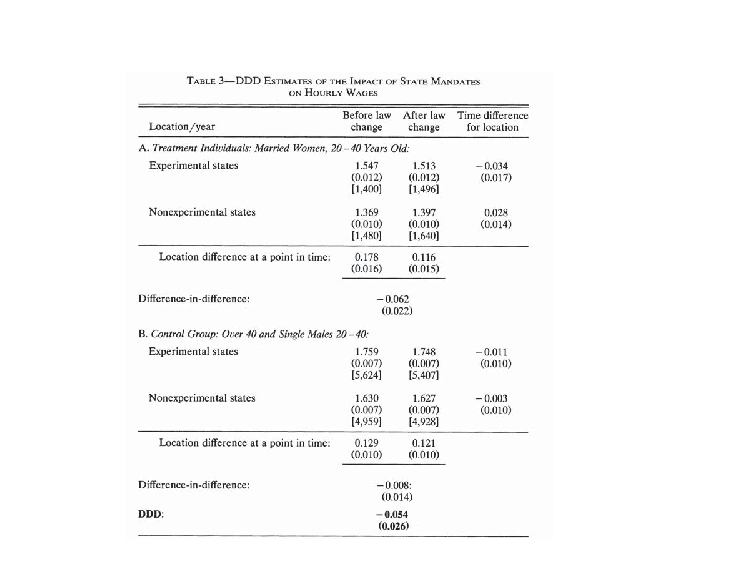
\includegraphics[width=0.92\linewidth,height=0.76\textheight,keepaspectratio]{figures/gruber_ddd_3.pdf}
	\end{figure}
	
\end{frame}

\begin{frame}{Triple differences commentary}

\begin{itemize}
\item Some people think that it requires that the placebo DiD be zero, but that's incorrect

\item In Gruber's 1995 article, it isn't clear why he needed triple differences in the first place -- his triple differences yielded -0.054 which is almost the same as what he found with his first diff-in-diff (-0.062)
\item The main value of triple differences is that you use it when you believe the parallel trends assumption doesn't hold

\end{itemize}

\end{frame}


\begin{frame}[shrink=20]

\begin{table}\centering
		\caption{Difference-in-Difference-in-Differences (Gruber version)}
		\tiny
		\begin{center}
		\begin{tabular}{lll|l|lll}
		\toprule
		\multicolumn{1}{l}{\textbf{Groups}}&
		\multicolumn{1}{c}{\textbf{States}}&
		\multicolumn{1}{c}{\textbf{Period}}&
		\multicolumn{1}{c}{\textbf{Outcomes}}&
		\multicolumn{1}{c}{$D_1$}&
		\multicolumn{1}{c}{$D_2$}&
		\multicolumn{1}{c}{$D_3$}\\
		\midrule
		&&After	&$NJ+MW+\textcolor{blue}{NJ_t}+\textcolor{red}{MW_t}+D$					\\
	&Experimental			&&&$\textcolor{blue}{NJ_t}+MW_t + D$			\\
		&states&Before	&$NJ+MW$					\\
Married women 					&&&&&$D+\textcolor{blue}{NJ_t} -PA_t 	$	\\
20-40							&&&&&$$\\
    		&&After	&$PA+MW+PA_t+MW_t$					\\
	&Non-experimental		&&	&$PA_t+MW_t$				\\
		&states&Before	&$PA+MW$					\\
								\\
&&&&&&$\textcolor{black}{D}$
\\
		&&After	&$NJ+SO+NJ_t+SO_t$				\\
	&Experimental 			&&&$NJ_t+SO_t$ \\				
		&states&Before	&$NJ+SO$					\\
Single men 					&&&&&$NJ_t  - PA_t$		\\
Older women					&&&&&$$		\\
	     	&&After	&$PA+SO+PA_t+SO_t$					\\
	&Non-experimental		&&&	$PA_t+SO_t$				\\
		&states&Before	&$PA+SO$					\\
		\bottomrule
		\end{tabular}
		\end{center}
	\end{table}

\begin{center}
\textbf{Triple diff assumption}
\end{center}

$\widehat{\delta}_{DDD}= D + \underbrace{[(\textcolor{blue}{NJ^{MW}_t} - PA^{MW}_t) -( NJ^{SO}_t - PA^{SO}_t )]}_{\mathclap{\text{Equally biased  DiD \#1 and \# 2}}}$

\bigskip
Triple differences requires two diff-in-diff, from different groups, with the same bias. Parallel bias


\end{frame}







\begin{frame}{DDD in Regression}
	
	\begin{eqnarray*}
	Y_{ijt} &=&\alpha +  \beta_2 \tau_t + \beta_3 \delta_j  + \beta_4 D_i + \beta_5(\delta \times \tau)_{jt} \\
	&& +\ \beta_6(\tau \times D)_{ti} +  \beta_7(\delta \times D)_{ij} +  \textcolor{red}{\beta_8(\delta \times \tau \times  D)_{ijt}}+  \varepsilon_{ijt}
	\end{eqnarray*}
	
	\begin{itemize}
	\item Your dataset will be stacked by group $j$ and state $i$
	\item $\widehat{\beta_8}$ estimates the ATT
	\item Parallel bias, NA and SUTVA necessary and sufficient for identification
	\end{itemize}
	
\end{frame}



\begin{frame}{Simulation}

In /Labs/DDD I have a simulation to illustrate this for us called ddd2.do.  The ATT is -\$5,000 but the biased DiD is -\$7487.  The non-parallel trends bias is -\$2,487.  So I replicate Gruber (with simulated data) where the placebo DiD is close (-\$2,507).  I then present a triple differences which gives us -\$4,972. Let's look at the final product.

\end{frame}

\begin{frame}{Triple differences event study}

\begin{figure}
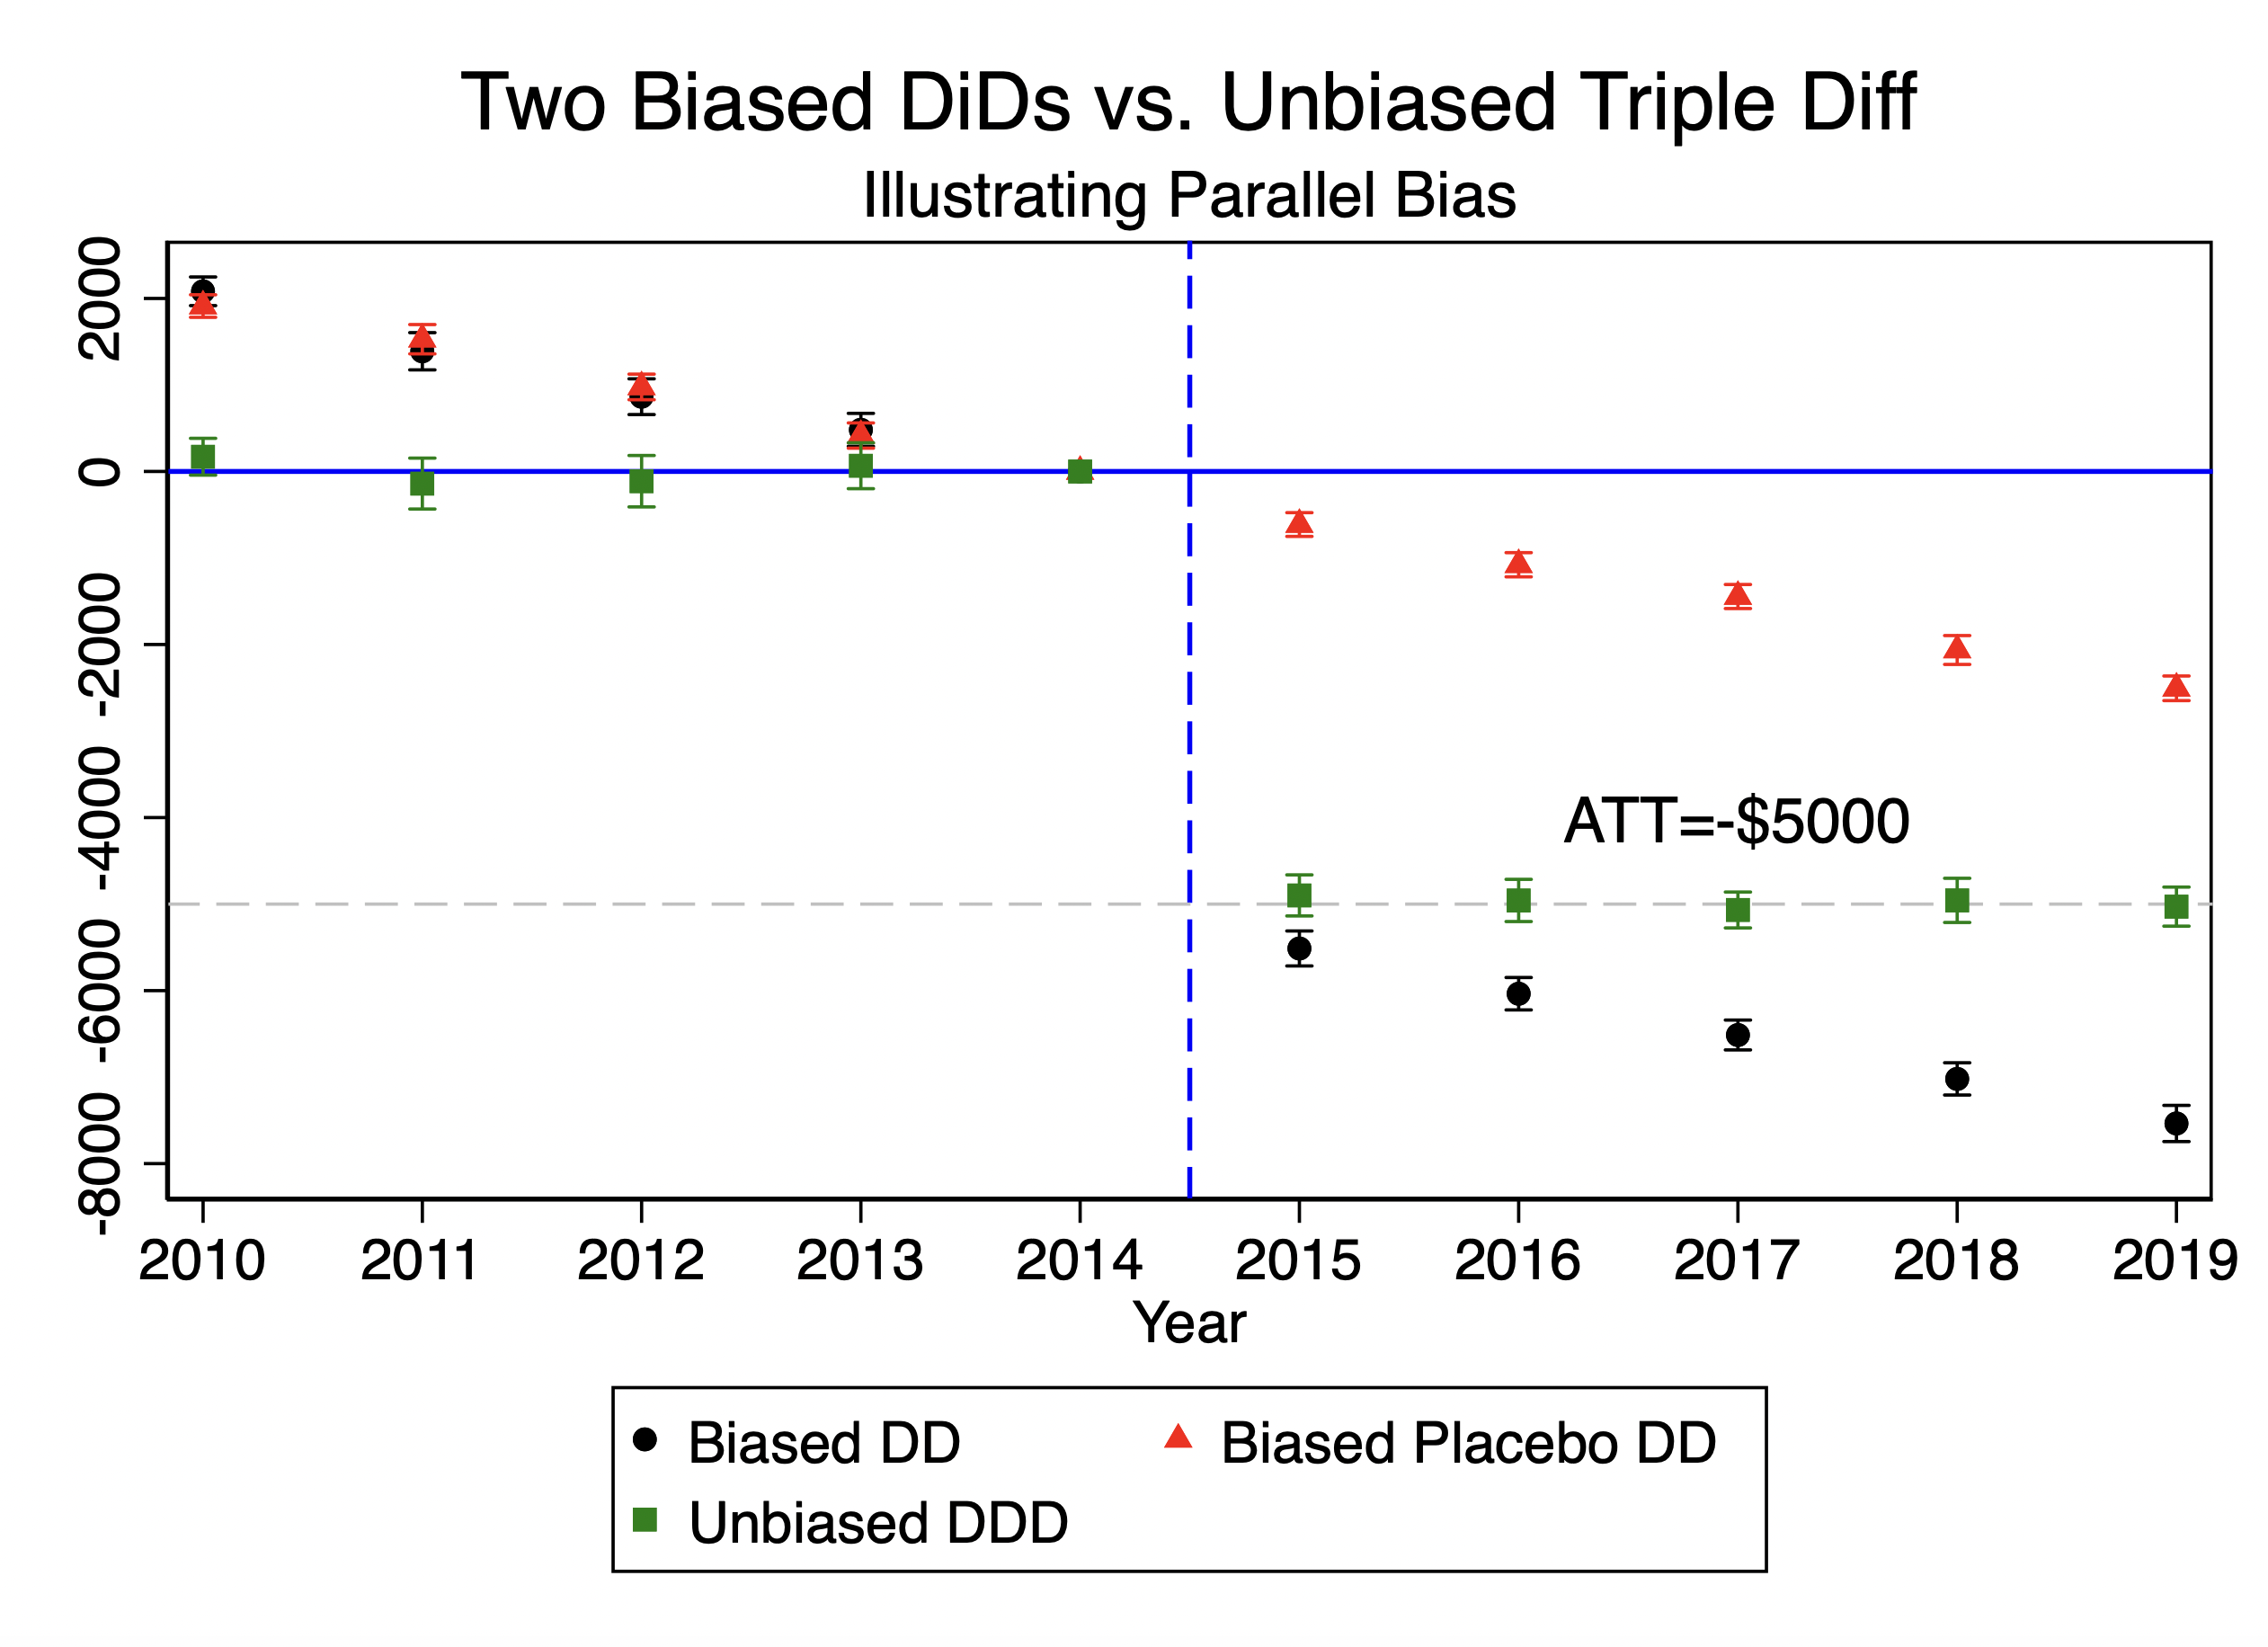
\includegraphics[width=0.92\linewidth,height=0.78\textheight,keepaspectratio]{figures/ddd_simulation}
\end{figure}



\end{frame}  

\begin{frame}{Great new paper to learn more}

\begin{figure}
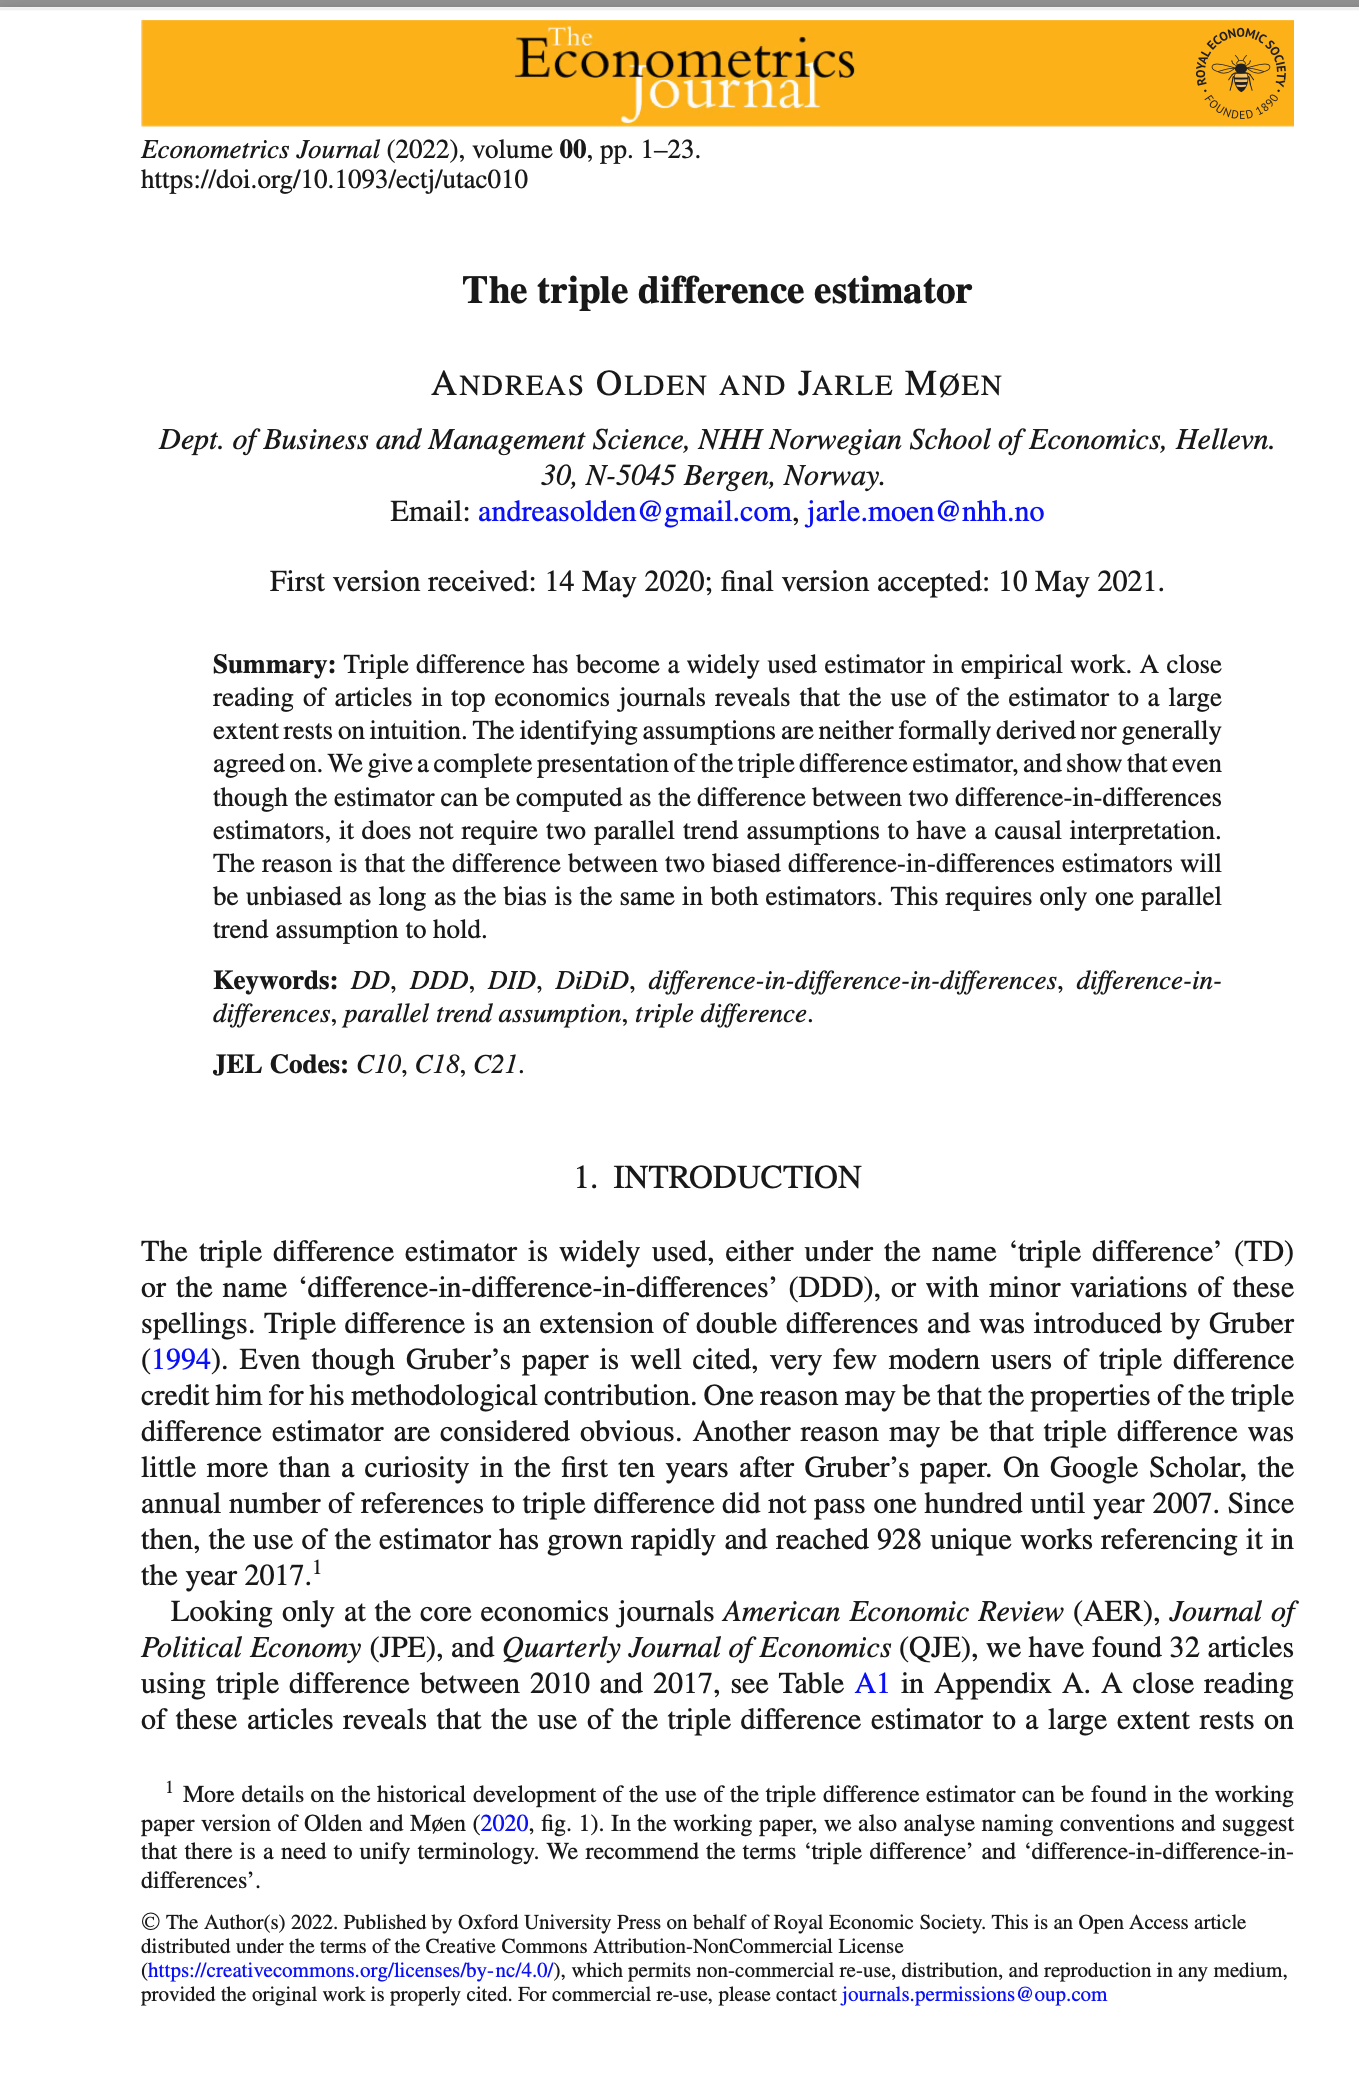
\includegraphics[width=0.88\linewidth,height=0.78\textheight,keepaspectratio]{figures/olden_moen_2022_ddd.png}
\end{figure}

\end{frame}


\begin{frame}{Summarizing DDD}

\begin{itemize}
\item Used to be people thought DDD required two parallel trends assumptions but it does not -- it is a real design and requires one parallel trends assumption
\item Parallel trends assumption is ``parallel bias'' -- that the bias of the true DiD is the same as the bias of the placebo DiD
\item The ladder of evidence still holds -- you'll want to present the event study plot, and my code provides it for you, because you need to evaluate the parallel bias assumption
\item Given the lack of triple diff literacy, you may have to write this anticipating reader and maybe editor confusion and so "educate" as you go -- overlaying all three plots could be help

\end{itemize}

\end{frame}

\end{document}
